\begin{figure}[!tb]
\begin{center}
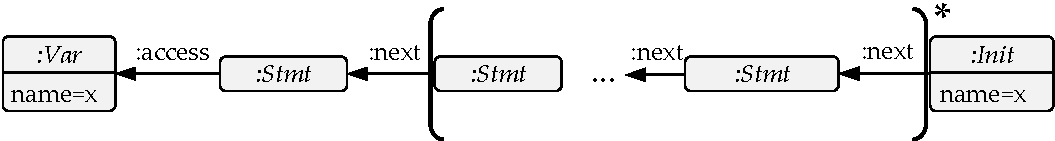
\includegraphics[width=.9\textwidth]{img/semantics/static.pdf}
\end{center}
\caption{Recursive Graph Constraint - ``Each variables is initialised before being accessed''}
\label{fig:sec-compl-static-sem:constraint}
\end{figure}

In the following, we focus on static semantics of models that can be expressed by (infinite) graph constraints on the structure of graphs by using the concept of recursive graph constraints from \cref{sec-dc-general-rec}.
For example, for abstract syntax trees of source code in \cref{sec-compl-software-trans}, we can define a recursive graph schema which leads to the infinite recursive graph constraint as indicated in \cref{fig:sec-compl-static-sem:constraint}.
The constraint expresses the requirement that each variable \code{Var} of \code{name} \code{x} that is \code{access}ed by some statement \code{Stmt} in the program has to be \code{Init}ialised before.
The path from the accessed variable to its initialisation is expressed by a regular path with an arbitrary number of statements in between by a recursive graph schema and induced infinite constraint.
By the construction in \cref{sec-dc-general-rec}, we can construct a finite graph constraint from the infinite one which then can be used within the verification of completeness of software transformations in \cref{sec-compl-software-trans}.